\subsection{Ground-Based Magnetometer}

\begin{wrapfigure}{r}{0.3\textwidth} 
\vspace{-30pt}
  \begin{center}
    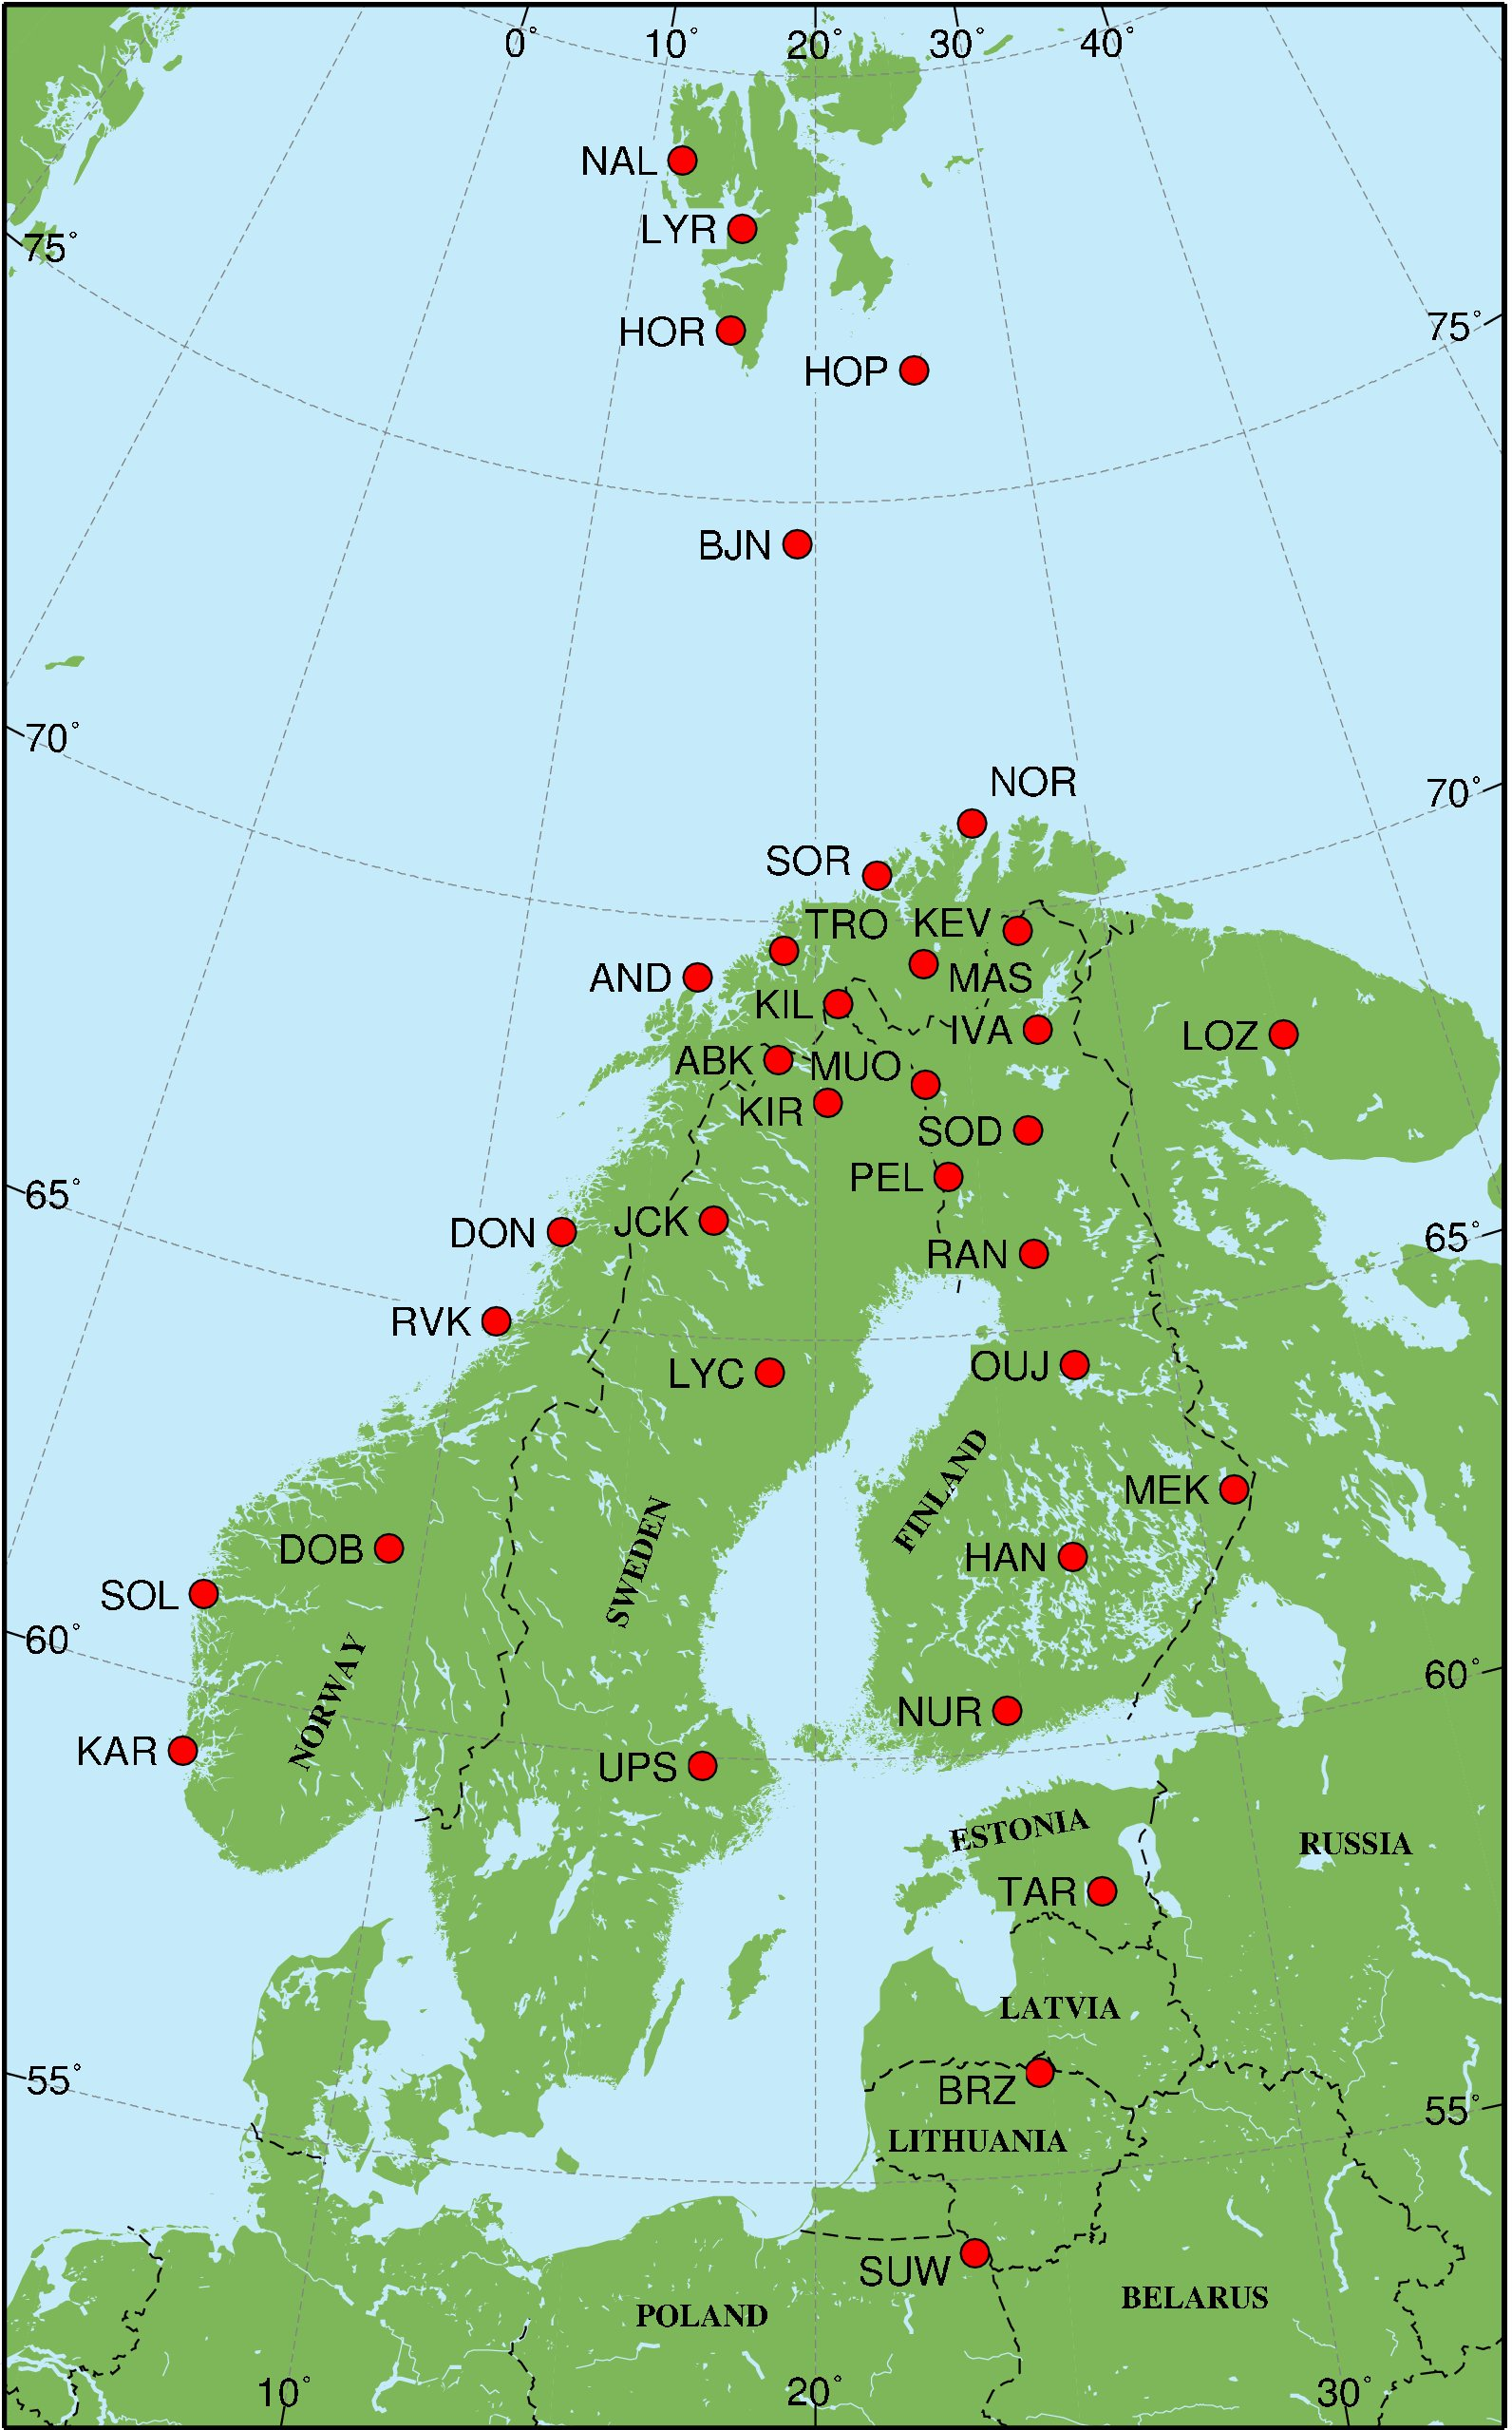
\includegraphics[width=0.2\textwidth]{Figures/Magnetogram/image_map_2015.jpg}
    \caption{The locations of the Magnetogram stations.}
    \label{fig:magnetogram}
  \end{center}
  \vspace{-30pt}
  \vspace{1pt}
\end{wrapfigure}
International Monitor for Auroral Geomagnetic Effects (IMAGE) are studying auroral electrojets and two dimensional current systems. It consists of 35 magnetometer stations in Finland, Sweden, Estonia, Norway and Russia. And is covering latitudes from 54 to 79 degrees north. 




